
\chapter{Wireless cameras introduction}
\label{chap:wifi-cam}

% \section*{Introduction}
% \label{sec:cam-intro}

Personal wireless surveillance cameras are widely available for a large public nowadays.
From hotel receptions to home surveillance or supervision of the babysitter\footnote{Miniature wireless cameras called \emph{nanny cam} are sold on specialised websites for the sake of child safety.}, many reason can justify the usage of a video camera.
While these cameras have valid usages, it is an open door to very important privacy threats.
The possibility for unauthorised people to access the video could have the opposite effect of protecting something (helping the work of potential burglars for example).
During the placing of this kind of wireless cameras, the question of security and privacy is often neglected or completely forgotten.\\

This chapter describes the different types of cameras and possible abuses on the web.
%The wireless cameras are divided in two types: analogical and digital cameras.

\section{Analogical cameras}
\label{sec:cam-analogic}

Analogical video cameras are often cheaper than the digital models and easier to install (no wifi network required).
This explains the fact they are still in use nowadays and may still be used in the future for shops and personal usages.
The video camera records analogical pictures and transmits it on a defined radio frequency.
To visualise the video, a receptor is set on the same frequency.
The frequency bands used are usually around 2,4GHz and have been selected as to avoid conflict with other emissions.\\

The important aspect about these cameras is the fact that, as the video is broadcasted on a defined frequency, any receptor set on this frequency can receive and watch the video stream.
This implies that there is technically no protection on the video stream.
Anybody using a portable receptor is able to watch the video stream (which could also contain an audio stream depending on the camera model) at a range of a few metres.\\

The usage of this type of camera should only be reserved for non sensible content and be considered as watchable by anybody.

\section{Digital cameras}
\label{sec:cam-digital}

Unlike the analogical video cameras, the digital models record digital images and transmit it using numerical stream, in this case, using wifi networks.
The protection of the video stream is then possible at several level:\\

\begin{itemizealt}
\item Encryption of the wireless network (WEP, WPA, WPA2...)
\item Encryption of the transmission protocol (usage of SSL to transmit the images)
\item Access control mechanism to the stream itself (password to access the admin interface)
\end{itemizealt}

The security of the video stream is then directly related to the choice of the security mechanism.
Using a weak security mechanism (for example WEP) leads to a weak security of the camera.\\

The digital video cameras can contain many features for the transmission of the video stream.
As these features improve the access convenience using different methods (admin interface, mail sending...), they also put a challenge on the side of the end user who must understand the key differences in term of security.
For instance setting an admin password to the administration interface during the configuration process does not protect the RTSP\footnote{RTSP, for \emph{Real Time Streaming Protocol}, is a streaming protocol, often used to embed the video stream in third party softwares.} stream in the analysed D-Link camera.

\section{Web digital cameras}
\label{sec:cam-google}

Some digital cameras are available on the Internet .
This section explains how a camera can be accessed from outside the local network and what are the risks of discovery and abuses.

\subsection{Connectivity}
\label{sec:cam-connect}

The default deployment of a digital camera is to be restricted to a home network using wifi.
%This is the default behaviour when a camera such the one studied in Chapter \ref{chap:cam-dcs} is connected on a wireless network. 
However, it is possible to make the video available on the Internet.
This is done by configuring a port forwarding at router level.
Then the public IP address of the network can be used to access the web interface of the camera.
Some camera systems also allow streaming to external websites or implements dynamic DNS mechanisms to be able to access the video stream from an URL.\\

Another common usage of web digital cameras is for outdoor cameras streaming streets, parks, ski resorts and other public areas.
Unlike previously mentioned personal cameras, these cameras may be published and advertised on city websites or neighbourhood associations.

\subsection{Google indexing}

If the URL to a web camera interface is published on a website (legitimate or not), it may be detected and indexed by a search bot software such as the ones Google uses to constitute its search engine database.
If indexed, these cameras can be listed with the correct search keywords.\\

Using the Google search engine, the keyword \texttt{inurl:} is used to search in the site's URL itself.
On certain models of digital cameras, the URL to access the web interface contains some patterns typical of these cameras.
It is the case for example of \texttt{axis-cgi/mjpg} or \texttt{ViewerFrame?Mode=} that are present mostly in webcam server softwares.
Using the following search queries can list links to the web interface of digital cameras:

\begin{itemizealt}
\item \texttt{inurl:ViewerFrame?Mode=}
\item \texttt{inurl:ViewerFrame?Mode=Refresh}
\item \texttt{inurl:axis-cgi/jpg}
\item \texttt{inurl:axis-cgi/mjpg}
\item \texttt{inurl:view/indexFrame.shtml}
\item \texttt{inurl:view/index.shtml}
\item \texttt{inurl:view/view.shtml}
\end{itemizealt}

While these cameras are, most of the time, filming public areas were already available on websites without restrictions, these search queries allow quickly to list a large quantity of cameras.
By refining the search with other keywords such as \emph{airport} or the name of cities, it may make easier the collect and cross-checking information and facilitate abuses.\\

\subsection{Detection of non-public cameras}
\label{sec:cam-detection-hidden}

To end up in Google results, all the cameras have been published on a web page that was indexed by Google.
However, it is possible to find camera streams of more private areas such as bars, factories or even homes.
Most likely, these cameras have not been published by their owner on a website that was indexed by a search engine bot.
%If these digital cameras are not protected with an access control mechanism, anybody with the correct address can watch it.
Often, the owners of personal cameras rely on the fact that the IP address or URL to access these cameras are not known and published.
However it is possible to find and access the video stream of such cameras in some cases.
Two main methods can be used to detect these private cameras:\\

If a dynamic DNS system is used (some cameras integrate DDNS clients in their configuration), the URL address can have a form similar to http://\emph{\textless client-id\textgreater}.\emph{\textless ddns-provider\textgreater}.
This is the case for example with AXIS\footnote{AXIS \url{http://www.axis.com/}} surveillance cameras system which provides a dynamic DNS system URL with the form http://\emph{\textless client-id\textgreater}.axiscam.net.
By iterating or using a dictionary on common keywords, it is possible to find cameras that were not intended to be published.\\

Another method to detect cameras are to scan ranges of IPs addresses.
By iterating on a range of IP addresses, it is possible, with a sufficient amount of time, to list any type of IP device, including digital cameras, accessible via a public IP address.
Some cameras have unique patterns in the URL or in the header of the requests, searching for these patterns allow to detect these hidden cameras.
A script detecting the model of D-Link cameras studied in Chapter \ref{chap:cam-dcs} is described in Section \ref{sec:dcs-web-access}.\\

\subsection{Shodan}
\label{sec:shodanhq}

Shodan\footnote{SHODAN - Computer Search Engine \url{http://www.shodanhq.com/}} is a search engine targeted at finding online devices.
Instead of crawling the content of web pages, it scans IP ranges using headers, IP and ports to detect devices connected to the Internet.\\

In the case of camera, this search engine can be used to detect web cameras available on the Internet.
The case where a camera interface is not protected using an access control mechanism, people using Shodan may find it and be able to watch the video stream.
The usage of an access control mechanism does not prevent the indexing of a camera by Shodan but helps to avoid unauthorised accesses.
Figure \ref{fig:shodan-dcs} shows an example of a search done to find D-Link DCS-2130 camera, finding 195 devices.

\begin{figure}[h]
  \centering
  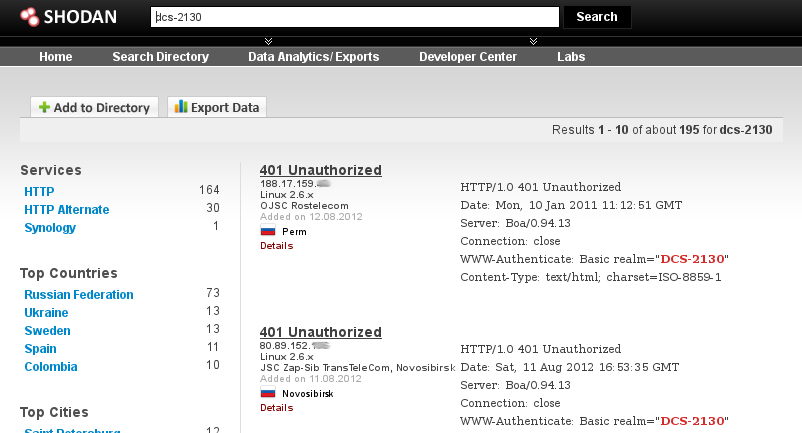
\includegraphics[width=\textwidth]{images/shodan-dcs.png}
  \caption{Shodan search to find D-Link DCS-2130 camera}
  \label{fig:shodan-dcs}
\end{figure}

\subsection{TRENDnet vulnerability}
\label{sec:trendnet-hack}

While the methods mentioned previously abuse from a lack of protection, some cameras, even protected, suffer from vulnerabilities and the video stream can be accessed if they are published on the web.
This is the case of a set of TRENDnet IP cameras on which a bug has been discovered.\\

In January 2012, the author of the webblog Console Cowboys, has published some researches he made about a TRENDnet digital camera~\cite{trendnet-hack}.
Through his researches, he discovered on the server, the presence of an executable binary file \texttt{mjpg.cgi} in a public cgi directory.
When executed, this file generates a video stream with regular snapshots of the camera.
By accessing the file through the URI \texttt{/anony/mjpg.cgi}, any user, even unauthenticated, would receive the video stream from any TRENDnet camera using this firmware as the example in Figure \ref{fig:trendnet-hack} shows.\\

\begin{figure}[h]
  \centering
  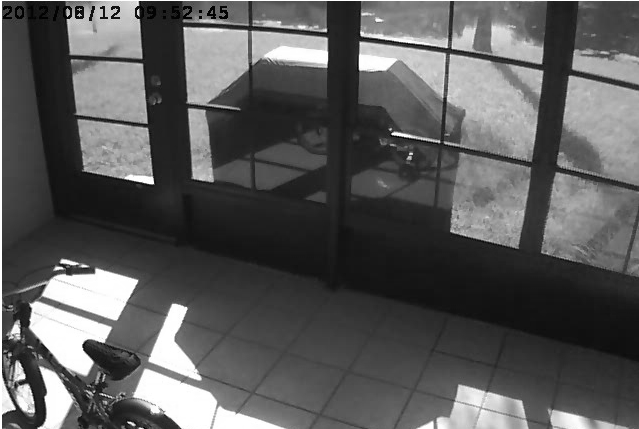
\includegraphics[width=7cm]{images/trendnet-hack2.png}
  \caption{Example of video stream accessed on a vulnerable camera}
  \label{fig:trendnet-hack}
\end{figure}

The exploitation of this vulnerability is made easier by the existence of the Shodan search engine presented in Section \ref{sec:shodanhq}.
Using the query \texttt{netcam} which is used in the headers of TRENDnet cameras, the Shodan search engine lists IP addresses of TRENDnet cameras.
Using this list, the vulnerability can be tested on a large number of devices.\\

TRENDnet replied to this publication by proposing an update of the firmware that fixes the vulnerability and contacting registered owners to warm them about the potential threat.
However it is very likely that most of the vulnerable devices will not be updated by their owners and still be exploitable in the future.\\

This vulnerability is an example of the danger of setting up such devices on the web.
Even by protecting correctly and not publishing the URL to access the camera, owners of these devices are exposed to any curious eyes as for the moment their camera is made accessible from the Internet.
Unlike the results from the Google Search in Section \ref{sec:cam-google}, these cameras are often personal cameras and are often used in private areas.
A similar bug permitting the access to the log file on the studied camera has been discovered and is explained in Section \ref{sec:dcs-log}.
